
\documentclass[utf8]{XDBAthesis}
% 图形文件的搜索路径
\def\allfiles{}
\def\pictures{}
\graphicspath{{figure/}}
\numberwithin{algorithm}{chapter}
\floatname{algorithm}{算法}
\renewcommand{\algorithmicrequire}{\textbf{输入:}}
\renewcommand{\algorithmicensure}{\textbf{输出:}}
%\usepackage[nomarkers]{endfloat}

\begin{document}
\lstdefinestyle{customc}{
  belowcaptionskip=1\baselineskip,
  breaklines=true,
  frame=single,
  xleftmargin=\parindent,
  showstringspaces=false,
  basicstyle=\footnotesize\ttfamily,
  keywordstyle=\bfseries\color{green!40!black},
  commentstyle=\itshape\color{purple!40!black},
  identifierstyle=\color{blue},
  stringstyle=\color{orange},
}

\lstset{numbers=left,
extendedchars=false,
escapechar=@,style=customc
}
%%----------------- 封面部分 ----------------- %%
    \class{031111}
    \schoolnumber{03111047}
    \title{手机拍照手势识别算法}{}   %%题目超过14个字把剩下的放到第二个空
    \college{计算机学院}
    \major{计算机科学与技术}
    \author{吕莹}
    \advisor{郭杏莉}
    \maketitle
%%----------------- 前言部分 ----------------- %%
    
    \frontmatter
    \begin{abstract}
    Android操作系统在智能手机、车载系统、平板电脑等领域现在正发挥着越来越大的作用,稳定、开放且免费的Android操作系统也受到了各大厂商的喜爱。然而,如今拥有的人机交互方式仍有一定的局限性,这种局限性主要体现在人机交互的距离上。传统点触式的人机交互方式已不足以满足当今人们的需求,基于视觉的手势识别俨然已成为人机交互中的新研究方向。以手势直接作为输入,人机之间不再需要中间媒介,即不触摸到屏幕也可对手机进行操作。
    
文中首先介绍了 Android 系统和 OpenCV 库的背景及架构原理,论述了当前 Android设备的人机交互方式;详细讨论了移植 OpenCV 库并部署到 Android 系统中的方法,其中 OpenCV 库是作为支撑识别自然手势信息处理或进行其它开发的基础图像处理函数库;重点论述了基于 Android 平台实现自然手势识别系统的整体框架设计,以及组成系统的各个模块的设计与实现方法;详细介绍了当Opencv和照相机同时调用摄像头时的解决方法与实现。
    
最后,对自然手势识别系统进行了测试。此系统可以根据分类器识别用户的手势动作,然后做出相应的决策,测试结果符合实时性检测要求,整体运行达到了预期的效果。这种交互方式更符合用户的自然行为习惯,交互过程中用户只需通过手势来传达命令给Android 智能设备,随着这种非接触式人机交互技术的不断成熟与完善,它将成为Android 智能设备的一种主要操控方式。
    
\keywords{安卓操作系统\ \ \ \    OpenCV\ \ \ \     手势识别\ \ \ \     手势检测\ \ \ \    人机交互 }
\end{abstract}
\begin{englishabstract}
Android operating system in the smart phone, automotive systems, tablet PCs and other areas are now playing an increasingly important role, stable, open and free Android operating system has also been a favorite of the major manufacturers.Today, however, human-computer interaction has still some limitations which mainly reflected in the distance human-computer interaction.Traditional touch-type human-computer interaction has been insufficient to meet the needs of people today, gesture recognition based on vision has become an interactive new research directions.

This paper introduces the background and principles of Android system architecture and OpenCV libraries, it discusses the current human-computer interaction Android device; a detailed discussion of the transplant OpenCV libraries and deploy to Android system, wherein the OpenCV library is a natural gesture recognition support information processing or other development on the basis of image processing libraries; focuses on the overall framework based on the Android platform design natural gesture recognition systems, and design and implementation of the composition of the various modules of the system; the details of when and camera at the same time calling Opencv Workaround when the camera and implementation.

Finally, the natural gesture recognition system was tested. This system can identify the user's classification gestures, and then make the appropriate decisions, test results meet the requirements of real-time testing, the overall operation to achieve the desired effect. This interactive approach is more in line with the user's natural behavior, user interaction simply to communicate commands to the Android smart devices through gestures, with the mature and perfect such a non-contact interactive technology, it will become Android smart an apparatus main control methods.

\englishkeywords{Android OS\ \ \ \ OpenCV\ \ \ \ Hand Gesture Recognition \ \ \ \ Gesture Detection\ \ \ \ Human Computer Interaction}    
\end{englishabstract}

    \tableofcontents
%%----------------- 正文部分 ----------------- %%
    \mainmatter
    \pagestyle{content}
    \ifx\allfiles\undefined
\documentclass{XDBAthesis}
\def\pictures{}
\begin{document}
\else
\fi
\chapter{绪论}
\section{课题研究背景及意义}

在科技高速发展、研究层出不穷、需求不断更新的今天,外设硬件或屏幕触碰作为机械式输入设备,在某些方面来说,很难进行3D和高度自由的输入,这种交互方式对人们的日常生活来说并不方便,需要一个学习并且适应的过程。随着研究工作的更加深入,人们更多的开始关注人脸识别 \cite{erol2007vision,lee1995model}、人眼跟踪、人体跟踪与识别及手势跟踪与识别等更加符合人类习惯的人机交互技术。

“手势”在人机交互中,不单单具有生动、形象而且直观的特点,更具有很强的视觉效果\cite{何阳清2004基于几何特征的手势识别算法研究} ,因此手势完全可以作为一种交互手段。研究人机交互形式,人体语言与有声语言的融合,对于提高机器视觉,进而提高人机交互接口的实用性是非常有意义的。

随着人机交互技术的发展,最初的交互方式大部分是以实体按键方式控制智能设备,而现在更多的发展为以屏幕触控方式为主,甚至有些设备已经完全淘汰了实体按键的交互方式。然而,随着用户需求的不断提高以及开发者头脑风暴的创意不断增加,不仅仅传统按键被市场渐渐淘汰,目前主流的屏幕触控方式也不能完全满足用户需求,这些操作方式都有一定的局限性,主要体现在用户需要接触到设备才能够完成操作,因此手势识别突破了距离的限制,给用户带来了全新的体验。随着这种以非接触式自然手势操作技术在Android系统中逐渐发展成熟,必将带来一场全新的技术革命,为开发者开拓眼界,更新了思维模式,提升在现在的发展中,很多软件都与手势识别相结合,如红外设备、Kinect等。但是对于摄像头识别手势拍照系统并没有很成型的作品,在拍照过程中可能因为一手持手机,另一只手拿东西或其他原因对按键造成不便,能把 OpenCV 移植到 Android 平台上使用是对图像图像处理在了市场竞争力。对移动终端上方便的进行具有的巨大意义。因此在拍照过程中加入手势识别是很有发展空间与发展潜力的项目之一。

\section{课题研究现状}

\subsection{Android软件发展现状}

Android系统自推出以来,就以明显的优势逐渐扩大自大的市场份额,尤其在国外,其呼声日高,可谓是如日中天,正处于蓬勃发展的开拓阶段\cite{张华2012android}。据美国某市场调研机构2012年发布的一份最新报告显示。2012年一季度在美国,基于Android系统的智能手机的销售量已占据全美手机销售量的28\%份额,而大名顶顶的IPhone手机其市场份额紧追其后,占到21\%的市场份额,已经确定了Android系统的市场占有比。据业内人士分析,随着Android系统相应软件的不断开发应用,选择Android系统手机或者无线终端设备的人会越来越多,其市场霸主的地位在更新更好的系统出现之前是不可动摇的。

未来基于Android系统的应用软件将进入飞速发展的全新阶段。Android系统的应用绝不仅局限于手机产业,几年来其迅速扩张到相关领域,例如平板电脑、车载系统、电视STB、智能电器、智能会议系统等。如今,各IT厂商都在努力的研发前沿应用软件,以期在Android系统发展这一群雄逐鹿的关键阶段,占领更多的市场份额。

目前对Android的发展方向一类是偏向硬件驱动,一类是偏向软件应用\cite{张建平2013基于}。从目前的招聘需求来看,后者的需求最大,包括手机游戏、手机终端应用软件和其他手机应用软件的开发。随着各种移动应用和手机游戏等内容需求日益增加,也将激励大中小型手机应用开发商加大对Android应用的开发力度,因此Android人才的就业前景也非常广泛。几乎每一个android手机用户都是游戏的需求者,都是潜在的顾客,现今的android用户不过是冰山一角,随着android手机市场进一步壮大,游戏的市场容量将具备较大的增长空间,游戏开发者不会愁吃不饱,只会愁胃口不够大。

如今国内的Android开发还是主要以应用开发为主,主要分成3类:为企业开发应用、开发通用应用(放到Android Market或者其他App Market销售)以及游戏开发(放到Android Market或者其他App Market销售)\cite{许瑾2011基于} 。第一类开发者一般身处规模较大的公司,这些公司主要为自有品牌或者其他品牌设计手机或者平板电脑的总体方案。除了根据需求对系统进行定制外,更多的工作在于为这些系统编写定制的应用。第二类开发者,一般处于创业型公司或者是独立开发者,他们的盈利方式主要是2种:为国外公司进行外包开发,或者通过Google的移动广告(AdMob)通过广告点击分成。而理论上的通过付费下载的形式来盈利的,现在国内鲜见成功者。第三类开发者,目前和第二类开发者类似。

丰富的应用软件程序有游戏、生活、新闻、阅读器、记事本、天气预报、文件或行事历管理及硬件管理方面的服务软件,而工具型软件将随着Android 系统日趋完善而减少,除了 UI 客制化及动作感测等结合硬件及软件的应用外,扩增实境应用也将逐渐进入 Android 应用领域中,更是值得关注的发展方向之一。

\subsection{手势识别研究现状}

手势是人类沟通交流不可分割的一部分:人们在相互交流时总会指手划脚。而手势识别技术又开辟了我们与机器、设备或电脑互动的新局面。手势识别的前景非常令人期待,特别是对于智能手机和平板电脑而言。这些设备已经深入人们生活的各个方面,而新的通信接口始终非常受人们的欢迎。

采用摄像头跟踪进行手势识别的技术实际上已经使用了一段时间。领先的游戏机,如微软的Xbox和索尼公司的Play Station,都配置了手势识别设备(分别是KINECT和Play Station Eye)。目前,这两种设备已经升级至第七代和第八代。不过,移动设备的手势识别技术仍面临几个重要问题,包括在不利的光线条件下,该技术能够实现的效果,背景的变化与高功耗等。然而,业内普遍认为,这些问题可以通过不同的跟踪解决方案和新技术克服。

这两年来智能移动终端设备特别是 Android 设备数量迅猛增长\cite{王赞超2013} ,很多开发者也将目光投降了除了触控以外其它的交互方式,例如语音识别技术,现在已日趋成熟,手势等肢体语言的交互形式将是另一个发展趋势,并有可能成为发展主体。近年来陆续出现了一些使用肢体语言交互的应用,如眨眼拍照的相机应用、笑容触发的相机应用、眼球转动来控制的阅读器应用等。相比之下更直观的手势交互应用必将成为热门。

\section{论文主要内容安排}

本论文共分为六章,内容安排如下:
\begin{itemize}
    \item 第一章:绪论。本章主要介绍了课题研究背景及意义、Android软件发展现状及手势识别的发展现状。
    \item 第二章:相关知识。本章介绍了Android平台,NDK,OpenCV和常见的图像处理方法,为后文详细叙述算法打下基础。
    \item 第三章:关键技术。本章主要介绍了算法过程中的几个关键技术,包括图像预处理技术(灰度处理,平滑处理),手势特征提取技术(Canny检测轮廓,直线检测等等)还有相机线程冲突的解决方案。由于本算法中我们为了加速运算,用到了部分C语言,所以最后还介绍了Android平台下C和Java的交叉编译方法。
    \item 第四章:算法设计与实现。本章详细介绍了算法的设计与实现,从手势选取方案到算法具体流程,再到最后的封装结果。
    \item 第五章:Demo实现与实验结果。本章给出了Demo的测试环境,框架结构,实现上的关键难点和实验结果。
    \item 第六章:总结与展望。本章总结了本文的主要工作,说明了具体的研究成果与不足,给出了下一步的工作方向。
\end{itemize}

\ifx\allfiles\undefined
%\bibliographystyle{unsrt}
\bibliography{main}
\end{document}
\fi
    \ifx\allfiles\undefined
\documentclass{XDBAthesis}
\def\pictures{}
\begin{document}
\else
\fi
\chapter{相关知识}

\section{Android平台}

\subsection{Android起源及发展状况}

\emph{Android}一词最早出现于法国作家利尔亚当在1886年发表的科幻小说《未来夏娃》中。他将外表像人的机器起名为Android。2010年2月3日,Linux内核开发者Greg Kroah-Hartman将Android的驱动程序从Linux内核“状态树”(“staging tree”)上除去,从此,Android与Linux核心开发分道扬镳。

Android是Google开发的基于Linux平台的开源手机操作系统\cite{单李旺2009android} 。它该平台由操作系统、中间件、用户界面和应用软件组成,是一个全面整合的软件栈,号称是首个为移动终端打造的真正开放和完整的移动软件平台。you谷歌与开放手机联盟合作开发了 Android,这个联盟由包括中国移动、摩托罗拉、高通、宏达和 T-Mobile在内的30多家技术和无线应用的领军企业组成。通过与运营商、设备制造商、开发商和其他有关各方结成深层次的合作伙伴关系,我们希望借助建立标准化、开放式的移动电话软件平台,在移动产业内形成一个开放式的生态系统。我们认为此举必将推进更好、更快的创新,为移动用户提供不可预知的应用和服务。

Android作为谷歌企业战略的重要组成部分,将进一步推进"随时随地为每个人提供信息"这一企业目标的实现。由数据表明,全球为数众多的移动电话用户从未使用过任何基于Android的电话。谷歌的目标是让移动通讯不依赖于设备甚至平台。出于这个目的,Android将会将其补充,而不会替代谷歌长期以来奉行的移动发展战略:通过与全球各地的手机制造商和移动运营商结成合作伙伴\cite{罗翔2010symbian} ,开发既有用又有吸引力的移动服务,并推广这些产品。开放手机联盟的成礼和Android的推出是对现状的重大改变,在带来初步效益之前,还需要不小的耐心和高昂的投入。但是,我们认为全球移动用户从中能获得的潜在利益是值得付出这些努力的。如果你也是一个开发者,并对我们的想法感兴趣,就请再给我们一星期的时间,届时谷歌便能提供SDK了。

Google与开放手机联盟(Open Handset Alliance)合作开发了Android移动开发平台,这个联盟由摩托罗拉、高通、宏达电和T-Moblie、中国移动等在内的30多家移动通讯领域的领军企业组成。Google与运营商、设备制造商、开发商和其他第三方结成了深层次的合作伙伴关系,希望通过建立标准化、开放式的移动电话软件平台,在移动产业内形成一个开放式的生态系统。    

Android作为Google企业战略的重要组成部分,将进一步推进“随时随地为每个人提供信息”这一企业目标的实现。全球为数众多的移动电话用户从未使用过任何基于Android的移动通讯设备,Google的目标是让移动通讯不依赖于设备甚至平台。出于这个目的,Android将补充而不会代替Google长期以来奉行的移动发展战略:通过与全球各地的手机制造商和移动运营商结成合作伙伴,开发即有用又有吸引力的移动服务,并推广这些产品。

\subsection{Android平台及其优点}

Android是开源的,开源是一种的完全开放的开发模式,有着很多移动终端平台的优点,主要有以下几点:
\begin{enumerate}
    \item 简单性

开源软件解决方案很容易找到和很容易实施,许多架构师和开发人员都熟悉这个技术的架构。开源软件团体推动开源软件开发人员提供使用方便的 框架和平台。开源软件解决方案还能够让企业迅速创建一些解决方案以提供有形的和可衡量的好处。
    \item 开放性
 
    
开源软件本身的灵活性允许比专有软件产品更大的自由和个性化。这就意味着一个机构能够从开源软件的安装中看到与自己的业务关系更密切 的更大的价值。 
    \item 价格负担低

Android是一款基于Linux平台的开源操作系统,从而避开了阻碍市场发展的专利壁垒,是一款完全免费的智能手机平台。而WindowsMobile高达20多美元的单台授权费相比,采用Android系统的终端可以有效的降低产品成本;Android系统对第三方软件开发商也是完全开放和免费的。Android系统承载着Google帝国的梦想。
    
\end{enumerate}





\subsection{Android系统架构原理}

    对操作系统而言,必须做到设计合理、层次分明,同时还需考虑整个系统的结构要聚耦适当,Android系统是基于Linux内核的,因此还必须具备开源的特性,以符合开源人员共同工作。 

    从系统的组成要件来讲,Android平台架构包括硬件设备、板级支持包、驱动程序、操作系统内核、程序运行库,运行框架,应用程序等,它们的有机结合和协同工作共同完成了整个系统的正常运行和对事务的处理。 

    依据Google开源资料可知\cite{王茜2011Android} ,整个系统由Linux内核、程序库、Android Runtime、应用程序框架和应用程序等5部分组成,系统架构如图\ref{fg:android}所示。
\begin{figure}[htb]
    \centering
    \includegraphics[width=0.8\textwidth]{figure/android}
    \caption{Android系统架构图}
    \label{fg:android}        
\end{figure}
    

参照图\ref{fg:android} ,由上而下对组成系统各部分的主要组件作以下描述。
\begin{enumerate}
    \item Linux内核 

    Android基于Linux 2.6内核,但并非完全照搬内核,而是对内核作了部分增删和修改,在Linux 2.6内核的基础上,Android核心系统实现了安全性、内存管理、进程管理、网络协议栈和驱动模型等功能,Linux内核也同时作为硬件和软件栈之间的抽象层。
    
    硬件驱动程序:完成与各种硬件的通信,Linux内核提供了大部分设备的驱动程序,如显示屏,摄像头,内存,键盘,无线网络,音频设备,电源等组件。 

系统内存管理:对所有可用的内存进行统一编码管理,定义一整套内存定位,使用与回收的策略。 

系统进程管理:内核管理进程的创建与销毁,管理进程间的通信,以及采取必要的措施避免死锁等内容。 

网络管理系统:无线网络设备工作原理,内核掌控如何读取网络设备中的缓存数据。 
    \item 程序库

程序库是指可供使用的各种标准程序、子程序、文件以及它们的目录等信息的有序集合,Android包含一些C/C++库,Android系统中不同的组件通过应用程序框架可以使用这些库,以下是一些核心库: 

    Surface Manager:管理显示子系统,并且为多个应用程序提供2D和3D图层的无缝融合。

    Media Framework:基于OpenCORE的多媒体框架,支持多种常用的音频、视频格式文件的回放和录制,同时支持静态图像文件。 

    SQLite:一个对于所有应用程序可用,功能强劲的轻型关系型数据库引擎。 

    OpenGL ES:3D图形库,用于3D图形渲染,该库可以使用3D硬件加速。 

    FreeType:位图(Bitmap)和矢量(Vector)字体显示。 

    WebKit:支持Android浏览器和一个可嵌入的Web视图。 

    SGL:2D图形库,用于2D图形渲染。 

    LibC:一个从BSD继承的标准C系统函数库,它是专门为基于嵌入式Linux设备定制的。 

    
    \item Android运行库(Android Runtime)

    Android运行库包括两部分:一是核心库,二是自身的虚拟机。 

    核心库提供Java编程语言核心库的大多数功能。Dalvik虚拟机是Google专为Android开发的,比SunJava虚拟机的效率更高,功能也更为复杂,以更好的支撑Android平台,并拥有独立的版权。每一个Android应用程序都在自己的进程中运行,都拥有一个独立的Dalvik虚拟机实例, Dalvik虚拟机执行.dex的可执行文件,该格式文件针对小内存的使用进行了优化,同时虚拟机是基于寄存器实现的,所有的类由Java编译器编译,然后通过SDK中的相应工具转化成.dex格式,最后由虚拟机执行。
    \item 应用程序框架

 应用程序框架是指定义了一个应用程序运行所必须的全部功能组件,开发者也可以访问核心应用程序所使用的API框架。该应用程序的架构设计简化了组件的重用;任何一个应用程序都可以发布它的功能块,并且任何其他的应用程序都可以使用其所发布的功能块(应该遵循框架的安全性限制)。同样,该应用程序的重用机制也使用户可以方便地替换程序组件。
    \item 应用程序 

    Android系统发布时,会同一系列核心应用程序和常用程序一起发布,如常用的手机功能程序,包括语音电话、通讯录、短信收发、照相、话机设置等;数据应用程序,包括邮件工具,日程表,浏览器,地图导航等,以及Android Market上的各种应用程序;所有的应用程序都是使用Java语言编写。 
    
\end{enumerate}


\section{NDK简介}

   NDK 即 Native Development Kit,NDK 是 Google 发布的一系列开发工具集合,这个工具可以帮助 Android 应用程序开发者编译来自 C/C++语言编写的源代码,然后嵌入到他们自己的应用包中,供应用程序调用。Android 的虚拟机在应用程序的源代码中通过JNI调用方法实现本地代码。在内核层面,这意味着你的应用程序源代码可以用关键字native方式声明一个或多个方法,用于指出这些方法是通过本地代码方式实现的;另外你必须提供一个本地共享库包含上述用关键字native声明的方法的具体实现代码。这个库是要被打包到应用程序的apk文件中,而且库的命名也要跟Unix的规则,即lib<something>.so,将包含一个标准的JNI入口点。

   NDK 集成了交叉编译器,并提供了相应的MK文件隔离CPU、平台、ABI 等差异。MK文件相当于配置文件,开发人员在MK 文件中设置一些参数、欲编译的文件及编译特性的要求等,这样编译器就可以根据 MK 文件创建出动态库 so 文件。为了更好的与C/C++开发相结合,也在不断完善开发中,目前 NDK 提供了一些稳定 API 头文件声明,但是在功能上还是相当有限,包括 C 标准库(libc)、标准数学库(libm)、压缩库(libz)、Log库(liblog)。随着版本的不断升级,功能将越来越强大。

\section{OpenCV简介}

OpenCV是近年来推出的开源、免费的计算机视觉库,利用其所包含的函数可以很方便地实现数字图像和视频处理\cite{秦小文2011基于} 。同时利用面向对象的VC++ 6.0编程工具,用C++语言进行程序编写,大大提高了计算机的运行速度。本文首先阐述了OpenCV的特点以及结构,然后以平滑处理、图像形态学为例介绍了OpenCV在数字图像处理中的典型应用。OpenCV算法库为VC++编程处理数字图像提供了很大的方便,其必将成为图像视频处理领域的强有力的工具。

利用OpenCV视觉库,科研开发人员只需添加自己的编写程序,直接调用OpenCV中的函数即可实现,这样不仅降低了开发程序的难度,而且缩短了相关程序的开发周期。

\section{常见图像处理方法}
    在手势识别中有很多常用的图像操作,例如图像的剪切、图像的缩放、图像的旋转以及图像的亮度调整\cite{何阳清2004基于几何特征的手势识别算法研究} 。我们以\emph{Pixe1Array[x,y]}来表示原有图像的二维像素矩阵,原有图像的高度用H来表示,原有图像的宽度用\emph{W}来表示,用\emph{PjxelArrayNew[x,y]}来表示结果图像的二维像素矩阵,结果图像的高度为\emph{HNew},宽度为\emph{WNew}。

\subsection{图像的剪切}

    图像的剪切操作的函数原型为\emph{void CImage::eliplmage(eReet\&reet)},需
要输入的参数为要剪切的图像的具体的位置,即要剪切图像左上角的位置和右下角的位置。

假定要剪切图像左上角位置为\emph{(left,top)},右下角的位置\emph{(right,bottom)},那我们只需要调整图像的宽度为\emph{(righi-left)},调整图像的高度\emph{(bottom-top)},从图像的二维数组中提取左上角到右下角之间的数据。剪切后图像的数据可以表示为:
$$
    PixelArray[x,y] ,\ \ \ left\leq x \leq right \ \ \wedge\ \  top \leq y \leq bottom
$$
\subsection{图像的缩放}

    图像的缩放操作的函数原型为\emph{void CImage::CollapseOrExpandlmage(double dbRatioX,double dbRatioY)}\cite{殷涛2004基于几何矩的手势识别算法}。输入的参数为图像水平方向需要缩放的尺度以及图像垂直方向需要缩放的尺度。

假定水平方向缩放的比例为\emph{a},垂直方向缩放的比例为\emph{b},那么,缩放后图像的高度为\emph{bH},缩放后图像的宽度为\emph{aW},对于原有图像的任一点\emph{PixelArray[x,y]},在缩放后对应的像素为:
$$
    PixelArray[i,j] ,\ \ \ ax\leq i \leq a(x+1) \ \ \wedge\ \  by \leq j \leq b(y+1)
$$


    令\emph{CountArray[i,j]}为结果图像中点\emph{(i,j)}对应原有图像像素的计数,那么每次有点映射到点\emph{(i,j)}的像素时,将结果图像中点\emph{(i,j)}的像素值加上该原有图像点\emph{(x,y)}的像素值,并将\emph{CountArray[i,j]}加1。
$$
    PixelArrayNew[i,j]=PixelArrayNew[i,j]+PixelArray[x,y]
$$
$$
    CountArray[i,j]=CountArray[i,j]+1
$$

由于经缩放后,结果图像中的某一点的像素可能对应原有图像中的多个像素,所以对于这种情况需要对该点的像素求取平均值:
$$
    PixelArrayNew[i,j]=\frac{PixelArrayNew[i,j]}{CountArray[i,j]} %PixelArrayNew[i,j]/CountArray[i,j]
$$


    图像缩放操作可以用一个简单的示意图(图\ref{fg:ss})来表示:
    
\begin{figure}[htb]
    \centering
    \includegraphics[width=0.5\textwidth]{figure/suofang}
    \caption{缩放示意图}
    \label{fg:ss}
\end{figure}

\subsection{图像的旋转}

    图像的旋转在所有的通用操作中是最复杂的,它的函数原型为\emph{void CImage::Rotatelmage(double dbAngle)}。从中可以看出,传入的参数是需要旋转的角度,该角度以弧度值来表示,正数表示的是逆时针方向旋转,负数表示的是顺时针方向旋转。

旋转操作的示意图如图\ref{fg:roat}所示(逆时针旋转\emph{Q}度):
\begin{figure}[htb]
    \centering
    \includegraphics[width=0.5\textwidth]{figure/roat}
    \caption{旋转示意图}
    \label{fg:roat}
\end{figure}
      

图中细黑色的表示原来图像的范围,粗黑色的为旋转后图像的范围,虚线的为原来图像经旋转后在结果图像中的位置。

旋转操作首先需要判断该角度属于哪一个象限,不同的象限所使用的变换公式是不同的。假定输入的旋转角度为$\theta $,令$\theta_1 $为$\theta$经变换后在$[0,2\pi ]$之间的角度,令$\alpha $ 为$\theta $经变换后在$[0,\pi /2 ]$之间的角度,其中:
$$
\alpha =\left\{ 
    \begin{aligned}
       & \theta_1 &0 \leq \theta_1 \leq \pi /2 \\
       & \theta_1 -\pi &\pi /2 < \theta_1 \leq \pi\\
       & \theta_1 -\pi &\pi < \theta_1 \leq 3\pi /2\\
       & \theta_1 -3\pi /2 \ \ \ &3\pi /2 <\theta_1 \leq 2\pi 
    \end{aligned}
\right.
$$
令
$$
\begin{aligned}
NW&=Wcos\alpha +Hsin\alpha \\
NH&=Wsin\alpha +Hcos\alpha 
\end{aligned}
$$
对于原图像中的点$(x,y)$,在新图像中对应的坐标为$(x',y')$,那么
\begin{enumerate}
    \item $\theta $在第一象限时$$HNew=NH,WNew=NW$$
    $$
    \begin{aligned}
      x'&=xcos\alpha +ysin\alpha\\
      y'&=(W-x-1)sin\alpha +ycos\alpha
    \end{aligned}
    $$
    \item $\theta $在第二象限时$$HNew=NW,WNew=NH$$
    $$
    \begin{aligned}
      x'&=(W-x-1)sin\alpha +ycos\alpha\\
      y'&=NW-1-xcos\alpha -ysin\alpha
    \end{aligned}
    $$
    \item $\theta $在第三象限时$$HNew=NH,WNew=NW$$
     $$
    \begin{aligned}
      x'&=NW-1-xcos\alpha -ysin\alpha\\
      y'&=NH-1-(W-x-1)sin\alpha -ycos\alpha
    \end{aligned}
    $$
    \item $\theta $在第四象限时$$HNew=NH,WNew=NW$$
     $$
    \begin{aligned}
      x'&=NH-1-(W-x-1)sin\alpha -ycos\alpha\\
      y'&=xcos\alpha +ysin\alpha
    \end{aligned}
    $$
\end{enumerate}
这样在任意的旋转角度下,原图像中的每一点都可以对应到新图像中的某一点中,考虑到经过旋转后在新图像中对应原图像部分的内部可能存在某些点在原图像中不存在对应点,所以需要对这些点作平滑处理,使图像达到连续的效果。
假定对于图像中的任一点$PixelArrayNew[x,y]$,如满足条件:
$$
\begin{aligned}
    PixelArrayNew[x,y] \ \ &\wedge\ \  \\
    PixelArrayNew[x-1,y]\neq 0 \ \ &\wedge\ \ PixelArrayNew[x+1,y]\neq 0 \\
    PixelArrayNew[x,y-1]\neq 0\ \ &\wedge\ \ PixelArrayNew[x,y+1]\neq 0
\end{aligned}
$$
则
$$
\begin{aligned}
     PixelArrayNew[x,y]&=\\
    &(PixelArrayNew[x-1,y]+PixelArrayNew[x+1,y]\\
    &+PixelArrayNew[x,y-1]+PixelArrayNew[x,y+1])/4
\end{aligned}  
$$
\ifx\allfiles\undefined
%\bibliographystyle{unsrt}
\bibliography{main}
\end{document}
\fi
    \ifx\allfiles\undefined
\documentclass{XDBAthesis}
\def\pictures{}
\begin{document}
\else
\fi
\chapter{关键技术}
本章将介绍本算法中的几个关键技术。


%\section{架构设计}
%
%    在已经搭建好了编译环境后,接下来主要进行两部分的开发:首先主要是涉及 UI 界面和程序的逻辑流程在基于Android应用程序框架下进行Java端的开发\cite{祝志远2015基于} ;其次是JNI接口的开发,通过OpenCV与JNI接口编写本地的 C/C++ 代码,并利用 Android NDK 对其进行编译,然后运用编译后生成的 Java 代码可调用动态链接库so文件,最后通过 Eclipse 编译打包并生成应用程序,整体框架图如图\ref{fg:whole}所示。
%\begin{figure}[htb]
%    \centering
%    \includegraphics[width=0.8\textwidth]{figure/opencv}
%    \caption{整体框架图}
%    \label{fg:whole}
%\end{figure}

\section{手势图像预处理}

\subsection{灰度处理}

在进行视频流目标识别与跟踪时,通常第一个步骤就是对采集到的彩色图像进行灰度化\cite{黄柏林2002基于边界特征的人脸识别},这是因为黑白照片数据量小,相比彩照更易实现实时算法,另一方面黑白照片是由未处理的光线所形成的照片,因此从图像处理学角度来看,这种未经特殊滤光处理的图片所涵盖的信息更有价值。

由于在OpenCV中自带函数可以实现图像灰度化,因此在该问题处理中直接调用函数\emph{:cvCreateImage}。实现代码如下。
\begin{lstlisting}[language=C]
cvNamedWindow("image",CV_WINDOW_AUTOSIZE );//创建窗口,窗口名字为image
cvShowImage("image",img);//在刚创建的image窗口中载入图像
//创建一个与img相同大小的图像img1
IplImage *img1 = cvCreateImage(cvGetSize(img),IPL_DEPTH_8U,1);
//色彩空间转换,将源彩色图像img转化成目标灰色图像imag1
cvCvtColor(img,img1,CV_BGR2GRAY); //关键
cvNamedWindow("GrayImage",CV_WINDOW_AUTOSIZE);//创建窗口,窗口名字GrayImage
cvShowImage("GrayImage",img1);//载入转化后的图像
cvSaveImage("/lena_gray.jpg",img1,0);
\end{lstlisting}
%
%
% \begin{figure}[htb]
%    \centering
%    \includegraphics[width=\textwidth]{figure/hui}
%    \caption{灰度处理实现代码}
%    \label{fg:hui}
%\end{figure}

\subsection{平滑处理}

消除图像中随机噪声的技术。对平滑技术的基本要求是在消去噪声的同时不使图像轮廓或线条变得模糊不清。常用的平滑方法有中值法、局部求平均法和k 近邻平均法。局部区域大小可以是固定的,也可以是逐点随灰度值大小变化的。此外,有时应用空间频率域带通滤波方法。

对于平滑处理,在OpenCV函数库中也有相应的函数\cite{王昭威2013基于}:

\emph{CV\_BLUR\_NO\_SCALE} (简单不带尺度变换的模糊) - 对每个象素的 $param1\times param2$ 领域求和。如果邻域大小是变化的,可以事先利用函数 \emph{cvIntegral} 计算积分图像。

\emph{CV\_BLUR} (simple blur) - 对每个象素$param1\times param2$邻域 求和并做尺度变换 $1/(param1\times param2)$。

\emph{CV\_GAUSSIAN} (gaussian blur) - 对图像进行核大小为 $param1\times param2$ 的高斯卷积。

\emph{CV\_MEDIAN} (median blur) - 对图像进行核大小为$param1\times param1$ 的中值滤波 (i.e. 邻域是方的)。

\emph{CV\_BILATERAL} (双向滤波) - 应用双向 $3\times 3$ 滤波,彩色 $sigma=param1$,空间 $sigma=param2$。param1平滑操作的第一个参数。param2平滑操作的第二个参数。对于简单/非尺度变换的高斯模糊的情况,如果param2的值为零,则表示其被设定为param1。

\section{手势特征提取}

    特征提取是计算机视觉和图像处理中的一个概念。它指的是使用计算机提取图像信息,决定每个图像的点是否属于一个图像特征。特征提取的结果是把图像上的点分为不同的子集,这些子集往往属于孤立的点、连续的曲线或者连续的区域。

特征提取与选择一般分为三个步骤:特征形成、特征提取、特征选择。

特征形成  有信号获取或测量得到原始测量,之后处理后得到图像特征,这样的特征称作原始特征,如手势图像属于数字图像,它的原始测量是各点灰度值,但是这些测量不适于作为特征,还要经过计算产生一组原始特征。

     特征提取  原始特征的数量可能很大,或者说样本是处于一个多维空间中,通过映射(变换)将原始特征变换为较少的新特征,这个过程称作特征提取。映射后的特征又称作二次特征,它们是原始特征的某种组合,所以特征提取在广义上就是一种特征映射。如公式\eqref{eq:tt}所示。
\begin{equation}
    A:Y\rightarrow X
    \label{eq:tt}
\end{equation}

其中\emph{Y}是测量空间,\emph{X}是特征空间,\emph{A}称为特征映射,又称作特征提取器。

     特征选择  从原始特征中挑出一些最具有代表性和分类性最好的特征,这个过程称为特征选择,它可以起到降低特征空间维数的作用。

\subsection{Canny检测轮廓}

Canny边缘检测器利用Canny算子进行检测,是目前最精确的检测器,并且已经被大量运用于程序中。从目前看来,canny边缘检测在做图像轮廓提取 方面是最优秀的边缘检测算法。

canny边缘检测采用双阈值值法,高阈值用来检测图像中重要的、显著的线条、轮廓等,而低阈值用来保证不丢失细节部分,低阈值检测出来的边缘更丰富,但是很多边缘并不是我们关心的。最后采用一种查找算法,将低阈值中与高阈值的边缘有重叠的线条保留,其他的线条都删除。

函数如下:
\begin{lstlisting}[language=C]
int main() 
{ 
    Mat I=imread("../cat.png"); 
    cvtColor(I,I,CV_BGR2GRAY); 
                                                 
    Mat contours; 
    Canny(I,contours,125,350); 
    threshold(contours,contours,128,255,THRESH_BINARY); 
    namedWindow("Canny"); 
    imshow("Canny",contours); 
    waitKey(); 
    return 0; 
} 
\end{lstlisting}
效果如图\ref{fg:Canny}所示。
\begin{figure}[htb]
    \centering
    \includegraphics[width=0.8\textwidth ]{figure/cat}
    \caption{Canny轮廓检测效果图}
    \label{fg:Canny}
\end{figure}


\subsection{直线检测}

直线在图像中出现的频率非常之高,而直线作为图像的特征对于基本内容的图像分析有着很重要的作用,我们通常通过OpenCV中的hough变换来检测图像中的线条。

首先展示最基本的Hough变换函数HoughLines,它的原型如下所示。
\begin{lstlisting}
void HoughLinesP(InputArray image, OutputArray lines, double rho, double theta,int threshold, double minLineLength=0, double maxLineGap=0 ); 
\end{lstlisting}
%\begin{figure}[htb]
%    \centering
%    \includegraphics[width=\textwidth]{figure/code}
%    \caption{HoughLines原型}
%    \label{fg:yuan}
%\end{figure}

 

    它的输入是一个二值的轮廓图像,往往是边缘检测得到的结果图像;它的输出是一个包含多个\emph{Vec2f}点的数组,数组中的每个元素是一个二元浮点数据对\emph{<rou,theta>}而言,\emph{rou}代表直线离坐标原点的距离,\emph{theta}代表角度。第3和第4个参数代表步长,因为\emph{Hough}变换实际上是一个穷举的算法,\emph{rho}表示距离的步长,\emph{theta}代表角度的步长。第5个参数是一个阈值设置直接的最低投票个数,知道\emph{Hough}原理的,这个参数应该很容易理解。

   从这个函数的输出结果我们可以看出,得到的直线并没有指定在图像中的开始点与结束点,需要我们自己去计算,如果我们想把直接显示在图像中就会比较麻烦,而且 会有很多角度接近的直线,其实它们是重复的,为了解决上面这些问题,\emph{OpenCV}又提供了一个函数\emph{HoughLinesP()}。它的输出是一个 \emph{Vector of Vec4i}。\emph{Vector}每一个元素代表一条直线,是由一个4元浮点数组构成,前两个点一组,后两个点一组,代表了在图像中直线的起始和结束点。

\subsection{轮廓的提取与描述}

在目标识别中,首先要把感兴趣的目标提取出来,而一般常见的步骤都是通过颜色或纹理提取出目标的前景图(一幅黑白图像,目标以白色显示在图像中),接下来要对前景图进行分析进一步地把目标提取出来,而这里常常用到的就是提取目标的轮廓。

OpenCV 里提取目标轮廓的函数是\emph{findContours},它的输入图像是一幅二值图像,输出的是每一个连通区域的轮廓点的集 合:\emph{vector<vector<Point>>}。外层\emph{vector}的\emph{size}代表了图像中轮廓的个数,里面\emph{vector}的\emph{size}代表了轮廓上点的个数。

提取到轮廓后,最重要的就是如何把这些轮廓转换为可以利用的特征,也就是涉及到轮廓的描述问题,这时就有多种方法可以选择,比如矢量化为多边形、矩形、椭圆等。OpenCV里提供了一些相应函数,在这里就不详细介绍了。 

\section{手势识别}
本算法中如何保证手势识别的准确度和速度是个尤为重要的问题。本节介绍了手势识别的具体过程。
\subsection{手势选取}
考虑到本算法为手势拍照设计的专用算法,故手势不需太多。为了保证识别性能,我们采用动态手势来作为算法识别的手势,即上划,下划,左划,右划四个基本手势。

\subsection{识别过程}


\section{照相机和Opencv同时对摄像头占用的处理方案}

    传统的处理方法是将图像一帧帧传入数据层,数据层调用图像处理函数完成对图像的处理后,再将图像传入表现层,使前端可以显示出当前图像。但是由于CPU有限,处理时间较长,会造成很明显的延时导致用户使用效果不理想。因此针对延时问题,采用多线程处理方案,当摄像头捕捉到图像后,对传入图像进行分频处理,即一帧传入数据层,一帧传入表现层。由于图像捕捉每一帧时间极短,因此在表现层也不会出现断帧的现象。分频处理不单单使画面更加流畅,还使软件在实时性的效果更好,图片处理更加快速。


\ifx\allfiles\undefined
%\bibliographystyle{unsrt}
\bibliography{main}
\end{document}
\fi
   % \ifx\allfiles\undefined
\documentclass{XDBAthesis}
\def\pictures{}
\begin{document}
\else
\fi
\chapter{图像处理及手势识别}

在手势识别中,处理的对象是手势的照片,我们提取数据的目标就是将手势的图像用一个特征向量来表示出来。在本文中所处理的图片主要有TIFF与BMP两种格式,TIFF格式相对来说要复杂一些,可以存储的图像也要丰富得多,它可以存储多张图片,还可以存储多种压缩格式的图片,而BMP格式的图片简单、通用,一般在应用程序中可以方便的显示。因此我们的工作除了熟悉多种格式的图像文件以外,还包括实现多种格式图像文件之间的相互转换,并最终提取出表示图像的特征向量。

\section{通用的图像操作}

    在手势识别中有很多常用的图像操作,例如图像的剪切、图像的缩放、图像的旋转以及图像的亮度调整。我们以\emph{Pixe1Array[x,y]}来表示原有图像的二维像素矩阵,原有图像的高度用H来表示,原有图像的宽度用\emph{W}来表示,用\emph{PjxelArrayNew[x,y]}来表示结果图像的二维像素矩阵,结果图像的高度为\emph{HNew},宽度为\emph{WNew}。

\subsection{图像的剪切}

    图像的剪切操作的函数原型为\emph{void CImage::eliplmage(eReet\&reet)},需
要输入的参数为要剪切的图像的具体的位置,即要剪切图像左上角的位置和右下角的位置。

假定要剪切图像左上角位置为\emph{(left,top)},右下角的位置\emph{(right,bottom)},那我们只需要调整图像的宽度为\emph{(righi-left)},调整图像的高度\emph{(bottom-top)},从图像的二维数组中提取左上角到右下角之间的数据。剪切后图像的数据可以表示为:



\subsection{图像的缩放}

    图像的缩放操作的函数原型为\emph{void CImage::CollapseOrExpandlmage(double dbRatioX,double dbRatioY)}。输入的参数为图像水平方向需要缩放的尺度以及图像垂直方向需要缩放的尺度。

假定水平方向缩放的比例为\emph{a},垂直方向缩放的比例为\emph{b},那么,缩放后图像的高度为\emph{bH},缩放后图像的宽度为\emph{aw},对于原有图像的任一点\emph{PixelArray[x,y]},在缩放后对应的像素为:



    令\emph{CountArray[i,j]}为结果图像中点\emph{(i,j)}对应原有图像像素的计数,那么每次有点映射到点\emph{(i,j)}的像素时,将结果图像中点\emph{(i,j)}的像素值加上该原有图像点\emph{(x,y)}的像素值,并将\emph{CountArray[i,j]}加l。

由于经缩放后,结果图像中的某一点的像素可能对应原有图像中的多个像素,所以对于这种情况需要对该点的像素求取平均值:



    图像缩放操作可以用一个简单的示意图(图\ref{fg:ss})来表示:
    
\begin{figure}[htb]
    \centering
    \includegraphics[width=0.5\textwidth]{figure/roat}
    \caption{缩放示意图}
    \label{fg:ss}
\end{figure}

\subsection{图像的旋转}

    图像的旋转在所有的通用操作中是最复杂的,它的函数原型为\emph{void CImage::Rotatelmage(double dbAngle)}。从中可以看出,传入的参数是需要旋转的角度,该角度以弧度值来表示,正数表示的是逆时针方向旋转,负数表示的是顺时针方向旋转。

旋转操作的示意图如图\ref{fg:roat}所示(逆时针旋转\emph{Q}度):
\begin{figure}[htb]
    \centering
    \includegraphics[width=0.5\textwidth]{figure/roat}
    \caption{旋转示意图}
    \label{fg:roat}
\end{figure}
      

图中细黑色的表示原来图像的范围,粗黑色的为旋转后图像的范围,虚线的为原来图像经旋转后在结果图像中的位置。

旋转操作首先需要判断该角度属于哪一个象限,不同的象限所使用的变换公式是不同的。假定输入的旋转角度为,令已为口经变换后在\emph{[0,]}之间的角度,令为经变换后在之间的角度,其中:


这样在任意的旋转角度下,原图像中的每一点都可以对应到新图像中的某一点中,考虑到经过旋转后在新图像中对应原图像部分的内部可能存在某些点在原图像中不存在对应点,所以需要对这些点作平滑处理,使图像达到连续的效果。

\section{手势图像预处理}

\subsection{灰度处理}

在进行视频流目标识别与跟踪时,通常第一个步骤就是对采集到的彩色图像进行灰度化,这是因为黑白照片数据量小,相比彩照更易实现实时算法,另一方面黑白照片是由未处理的光线所形成的照片,因此从图像处理学角度来看,这种未经特殊滤光处理的图片所涵盖的信息更有价值。

由于在OpenCV中自带函数可以实现图像灰度化,因此在该问题处理中直接调用函数\emph{:cvCreateImage}。实现过程如图\ref{fg:hui}。

 \begin{figure}[htb]
    \centering
    \includegraphics[width=\textwidth]{figure/hui}
    \caption{灰度处理实现代码}
    \label{fg:hui}
\end{figure}

\subsection{平滑处理}

消除图像中随机噪声的技术。对平滑技术的基本要求是在消去噪声的同时不使图像轮廓或线条变得模糊不清。常用的平滑方法有中值法、局部求平均法和k 近邻平均法。局部区域大小可以是固定的,也可以是逐点随灰度值大小变化的。此外,有时应用空间频率域带通滤波方法。

对于平滑处理,在OpenCV函数库中也有相应的函数:

\emph{CV\_BLUR\_NO\_SCALE} (简单不带尺度变换的模糊) - 对每个象素的 $param1\times param2$ 领域求和。如果邻域大小是变化的,可以事先利用函数 \emph{cvIntegral} 计算积分图像。

\emph{CV\_BLUR} (simple blur) - 对每个象素$param1\times param2$邻域 求和并做尺度变换 $1/(param1\times param2)$。

\emph{CV\_GAUSSIAN} (gaussian blur) - 对图像进行核大小为 $param1\times param2$ 的高斯卷积。

\emph{CV\_MEDIAN} (median blur) - 对图像进行核大小为$param1\times param1$ 的中值滤波 (i.e. 邻域是方的)。

\emph{CV\_BILATERAL} (双向滤波) - 应用双向 $3\times 3$ 滤波,彩色 $sigma=param1$,空间 $sigma=param2$。param1平滑操作的第一个参数。param2平滑操作的第二个参数。对于简单/非尺度变换的高斯模糊的情况,如果param2的值为零,则表示其被设定为param1。

\section{手势特征提取}

    特征提取是计算机视觉和图像处理中的一个概念。它指的是使用计算机提取图像信息,决定每个图像的点是否属于一个图像特征。特征提取的结果是把图像上的点分为不同的子集,这些子集往往属于孤立的点、连续的曲线或者连续的区域。

特征提取与选择一般分为三个步骤:特征形成、特征提取、特征选择。

特征形成  有信号获取或测量得到原始测量,之后处理后得到图像特征,这样的特征称作原始特征,如手势图像属于数字图像,它的原始测量是各点灰度值,但是这些测量不适于作为特征,还要经过计算产生一组原始特征。

     特征提取  原始特征的数量可能很大,或者说样本是处于一个多维空间中,通过映射(变换)将原始特征变换为较少的新特征,这个过程称作特征提取。映射后的特征又称作二次特征,它们是原始特征的某种组合,所以特征提取在广义上就是一种特征映射。如公式\eqref{eq:tt}所示。
\begin{equation}
    A:Y\rightarrow X
    \label{eq:tt}
\end{equation}

其中\emph{Y}是测量空间,\emph{X}是特征空间,\emph{A}称为特征映射,又称作特征提取器。

     特征选择  从原始特征中挑出一些最具有代表性和分类性最好的特征,这个过程称为特征选择,它可以起到降低特征空间维数的作用。

\subsection{Canny检测轮廓}

Canny边缘检测器利用Canny算子进行检测,是目前最精确的检测器,并且已经被大量运用于程序中。从目前看来,canny边缘检测在做图像轮廓提取 方面是最优秀的边缘检测算法。

canny边缘检测采用双阈值值法,高阈值用来检测图像中重要的、显著的线条、轮廓等,而低阈值用来保证不丢失细节部分,低阈值检测出来的边缘更丰富,但是很多边缘并不是我们关心的。最后采用一种查找算法,将低阈值中与高阈值的边缘有重叠的线条保留,其他的线条都删除。

函数如下:

效果展示:



\subsection{直线检测}

直线在图像中出现的频率非常之高,而直线作为图像的特征对于基本内容的图像分析有着很重要的作用,我们通常通过OpenCV中的hough变换来检测图像中的线条。

首先展示最基本的Hough变换函数HoughLines,它的原型如图\ref{fg:yuan} 所示。
\begin{figure}[htb]
    \centering
    \includegraphics[width=\textwidth]{figure/code}
    \caption{HoughLines原型}
    \label{fg:yuan}
\end{figure}

 

    它的输入是一个二值的轮廓图像,往往是边缘检测得到的结果图像;它的输出是一个包含多个\emph{Vec2f}点的数组,数组中的每个元素是一个二元浮点数据对\emph{<rou,theta>}而言,\emph{rou}代表直线离坐标原点的距离,\emph{theta}代表角度。第3和第4个参数代表步长,因为\emph{Hough}变换实际上是一个穷举的算法,\emph{rho}表示距离的步长,\emph{theta}代表角度的步长。第5个参数是一个阈值设置直接的最低投票个数,知道\emph{Hough}原理的,这个参数应该很容易理解。

   从这个函数的输出结果我们可以看出,得到的直线并没有指定在图像中的开始点与结束点,需要我们自己去计算,如果我们想把直接显示在图像中就会比较麻烦,而且 会有很多角度接近的直线,其实它们是重复的,为了解决上面这些问题,\emph{OpenCV}又提供了一个函数\emph{HoughLinesP()}。它的输出是一个 \emph{Vector of Vec4i}。\emph{Vector}每一个元素代表一条直线,是由一个4元浮点数组构成,前两个点一组,后两个点一组,代表了在图像中直线的起始和结束点。

\subsection{轮廓的提取与描述}

在目标识别中,首先要把感兴趣的目标提取出来,而一般常见的步骤都是通过颜色或纹理提取出目标的前景图(一幅黑白图像,目标以白色显示在图像中),接下来要对前景图进行分析进一步地把目标提取出来,而这里常常用到的就是提取目标的轮廓。

OpenCV 里提取目标轮廓的函数是\emph{findContours},它的输入图像是一幅二值图像,输出的是每一个连通区域的轮廓点的集 合:\emph{vector<vector<Point>>}。外层\emph{vector}的\emph{size}代表了图像中轮廓的个数,里面\emph{vector}的\emph{size}代表了轮廓上点的个数。

提取到轮廓后,最重要的就是如何把这些轮廓转换为可以利用的特征,也就是涉及到轮廓的描述问题,这时就有多种方法可以选择,比如矢量化为多边形、矩形、椭圆等。OpenCV里提供了一些相应函数,在这里就不详细介绍了。  


\ifx\allfiles\undefined
%\bibliographystyle{unsrt}
\bibliography{main}
\end{document}
\fi
    \ifx\allfiles\undefined
\documentclass{XDBAthesis}
\def\pictures{}
\begin{document}
\else
\fi
\chapter{软件实现与实验结果}
在第四章中提到了图像处理的基本方法与预处理方法,并且提及了手势特征的提取,本章将详细讲解算法在Android平台的实现并展示实验结果。

\section{算法总体设计}

本算法分为三个模块,手势检测模块、手势分割模块和手势识别模块,图\ref{fg:chart}显示了本算法软件设计的流程图。
\begin{figure}
    \centering
    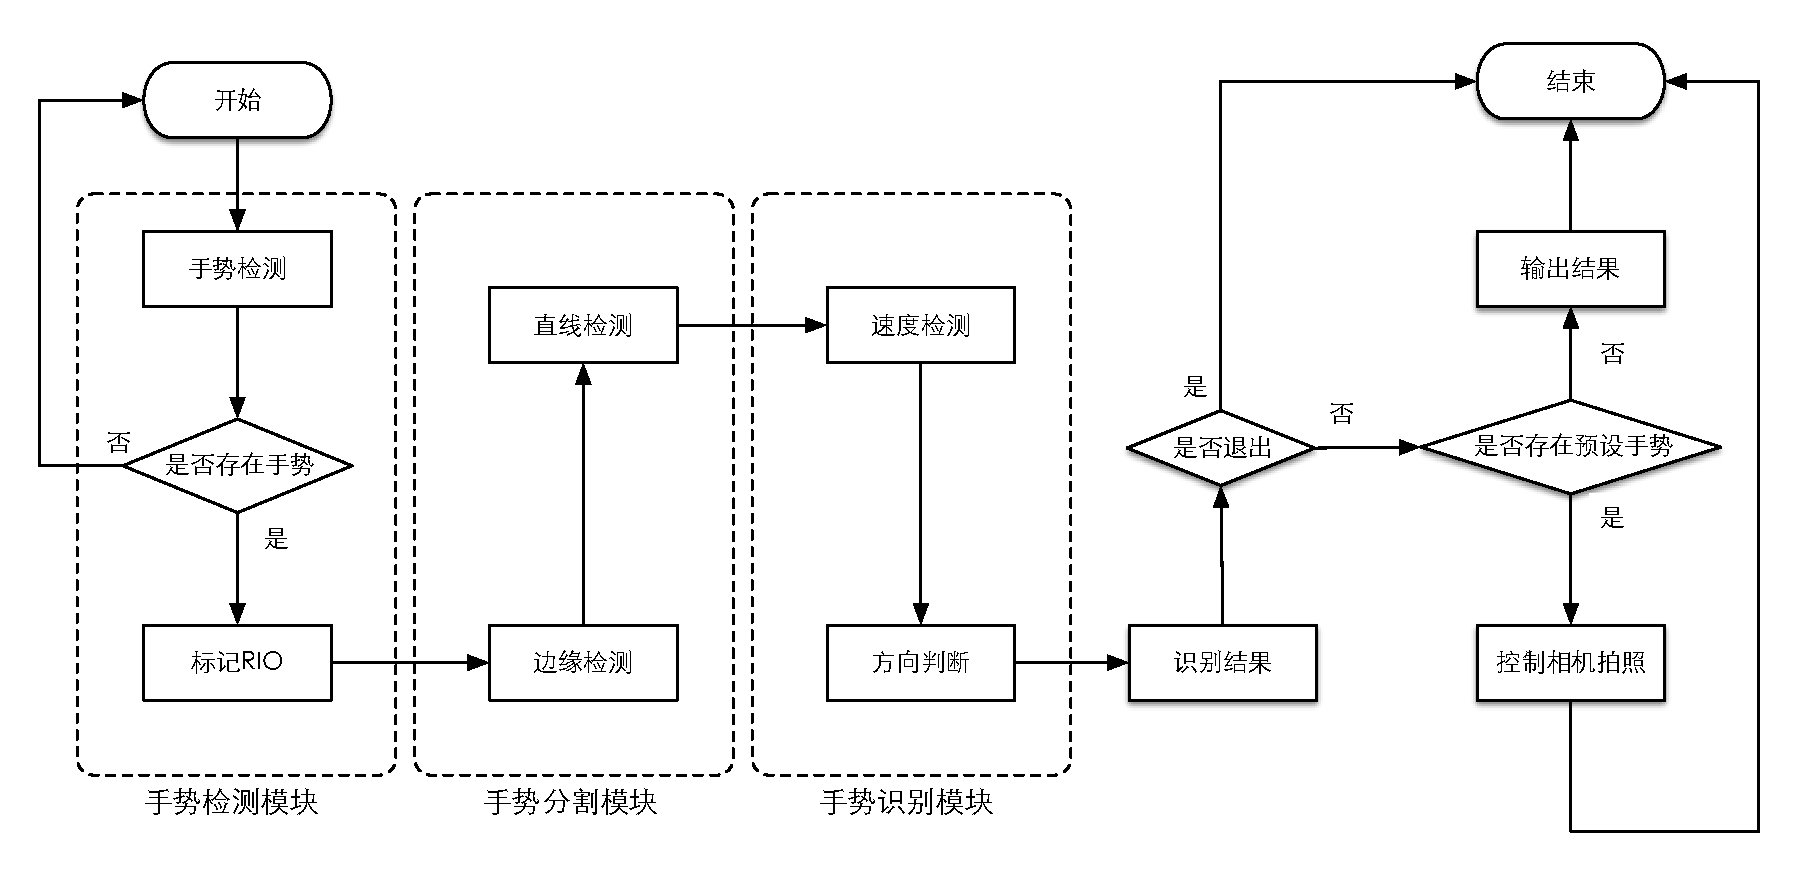
\includegraphics[width=0.9\textwidth ]{figure/chart}
    \caption{算法流程图}
    \label{fg:chart}
\end{figure}

在手势检测模块,实时检测视频流中的手势,标记检测到手势的区域为感兴趣区域;然后将感兴趣区域送入手势分割模块,利用直线检测对感兴趣区域进行处理,接着进行边缘检测和直线检测,得到手掌侧面的特征手势;在手势识别模块,对采集到的特征手势的运动进行判断,并增加时间限制,将对应的手势分别采取相对的处理机制。

\section{模块具体实现}

\subsection{手势检测模块}

功能实现使用Java语言利用OpenCV库编写了一个实时检测摄像头采集的视频流中手势的程序,抓取图片后进行灰度处理,当检测到手势时进入下一模块。

本实验是在较为复杂的背景下进行实验的,图中存在较多背景物体,同时有人脸存在,这些都没有影响到手势的正确检测,实验中仍然取得了很好的检测效果。

\subsection{手势分割模块}

    本算法采用的分割算法分为两个步骤:边缘检测和直线检测。将灰度处理过的图片采用Canny边缘检测算法,由于图片可能处理过仍有噪声,但是但是除手部以外的其他背景基本上完全滤除了,手掌形象也是清晰的。再采用直线检测,得到最终可识别的手势特征。

\subsection{手势识别模块}

在手势分割模块得到手势特征后,以移动距离为X轴,在单位时间内观察手势的运动走势并规定一定的速度范围内,手势动作最靠近哪种,就属于哪种手势识别,然后由上下左右动作分别对应指定的指令功能。
\section{软件运行结果展示}
我们利用本算法开发了个简单拍照demo,其主要功能是检测手动作,并进行相应操作:上划放大,下划缩小,左划倒计时3s拍照,右划倒计时5s拍照。
\subsection{手势识别在OpenCV上的实现}
图\ref{fg:1}为算法后台运行的log。可见,我们的算法采用间接抓取的方式,以16FPS的频率抓取图片,并处理展示。当识别到相应手势时现在log中显示,再进行相应操作。
\begin{figure}[htb]
    \centering
    \includegraphics[width=0.5\textwidth ]{figure/opencvframe}%
    \includegraphics[width=0.5\textwidth ]{figure/gesture}
    \caption{log记录}
    \label{fg:1}
\end{figure}
\subsection{CPU与系统内存占用}
CPU与系统内存占用如图\ref{fg:2}所示。可见,本算法对内存及计算量的要求并不算高,可以实际运用。
\begin{figure}[htb]
    \centering
    \includegraphics[width=0.5\textwidth ]{figure/cpu}%
    \includegraphics[width=0.5\textwidth ]{figure/memory}
    \caption{CPU与内存消耗占比图}
    \label{fg:2}
\end{figure}
\subsection{手势捕捉与处理}
当手势被识别后,进行对应功能处理。如果进入拍照功能,在屏幕右上角显示倒计时3秒,并在倒计时结束时拍照。如果是放大或缩小功能,由于前置摄像头无法实现物理变焦,故采用数字放大/缩小实现该功能。因为识别为动态过程,不方便截图展示,因此我们只截取了一个识别到左划手势并开始拍照倒计时的界面,和一个拍照完成的提示。如图\ref{fg:3}所示。
\begin{figure}[htb]
    \centering
    \includegraphics[width=0.3\textwidth ]{figure/recognize}%
    \includegraphics[width=0.3\textwidth ]{figure/capture}
    \caption{手势识别演示}
    \label{fg:3}
\end{figure}

%经过实验,我们可知在准确度,速度,稳定性上本算法均以达到实用标准。本算法已具有实际使用的可行性。

\ifx\allfiles\undefined
%\bibliographystyle{unsrt}
\bibliography{main}
\end{document}
\fi
    \ifx\allfiles\undefined
\documentclass{XDBAthesis}
\def\pictures{}
\begin{document}
\else
\fi
\chapter{总结与展望}

基于视觉的手势识别长期以来都是人机交互领域研究的热点。本课题在近两年来智能移动终端设备爆炸式增长的大背景下,针对智能移动终端设备的特点,对手势的检测和识别方法做了深入研究,并选取 Android 智能平台为应用背景,设计了一个 Android 平台上的实时手势交互系统,这是在智能移动设备上研究人机交互手段所做出的新尝试,本文所做的主要工作和取得的成果主要以下有几点:
\begin{itemize}

\item 第一,在OpenCV调用摄像头与处理图像占用CPU方面进行的分频处理,使得在处理时间和效率上得到了大大的提高,并且直线检测的速度较快,计算量较小,和同类处理方式相比适合在移动设备上使用。

\item 第二,在手势识别方面,本文首先研究了手势分割技术,良好的手势分割是识别的前提,本文通过边缘检测和直线提取两个步骤得到了较好的手势分割效果。

\item 第三,在应用方面,本文设计了一个基于 Android 平台的实时手势识别系统,还演示了通过调用该库实现的一个使用特定手势控制摄像头完成拍摄的应用案例,这是研究智能终端设备上人机交互技术的一次新的尝试。
\end{itemize}

目前在识别过程仍有一些不足,归纳起来,造成错误识别的主要原因有以下两条:
\begin{itemize}
\item 第一,手势是3D的图像,实验中采用了2D的形式来表现3D图像,造成了一些手势信息的丢失,这是错误识别的主要原因。

\item 第二,获取的图像质量不高,背景中的景物比较复杂,这些由景物产生的像素对手势轮廓的提取造成了干扰,使最终的特征提取造成错误。

\end{itemize}
本课题在未来还可以在以下四个方面加以研究:
\begin{itemize}
\item 第一,在现有的手势检测基础上进行手势跟踪,本文没有研究手势跟踪的算法,但如果要达到更好的交互效果就应该加入手势跟踪。

\item 第二,降低软件的CPU和内存的占用率,目前完成的图像处理软件在这方面做得并不够好,占用手机的资源比较多。

\item 第三,实现图像亮度自动调整的功能,由于日常生活中由于曝光不足的照片很常见,亮度自动调整具有比较现实的意义。可以增加一些特定功能,比如针对现有的年轻人群对照片的要求,增加美白,瘦脸,瘦身等功能

\item 第四,完善 Android 手势拍照应用,进一步提高软件的稳定性和识别的准确性,使其在实际生活中具有实用性,争取将其应用发布到 Android 应用市场,供广大Android 设备用户使用。
\end{itemize}

\ifx\allfiles\undefined
%\bibliographystyle{unsrt}
\bibliography{main}
\end{document}
\fi
%    \appendix
%    \include{chapter/chap-req}

%%----------------- 附件部分 ----------------- %%
    \backmatter
    \ifx\allfiles\undefined
\documentclass{XDBAthesis}
\def\pictures{}
\begin{document}
\else
\fi
\begin{thanks}
转瞬间四年的大学生活即将结束,在即将走出校门迈入工作生活之际,回首这三年来的学习历程,我满怀一颗感恩之心,感谢一路走来给予我帮助的各位老师、同学和亲人。

首先,我想把最诚挚的谢意和深深的祝福送给郭杏莉老师。本论文是在郭老师的指导和关怀下完成的,在此对郭老师对我的指导表示诚挚的感谢。使我在学习能力上得到了充分的锻炼,她,严谨的治学精神,实事求是的研究作风,对事业充满热情的投入和勤奋工作的态度不时地感染着我,教育着我,激励着我在学习和生活中不断进取。

感谢我的家人和男朋友,他们一直给予我精神上的鼓励、物质上的支持、学习上的督促。他们是我克服困难、不断追求进步的精神支柱和动力源泉!

最后感谢参加论文评审和答辩的各位老师对本文的认真审阅。
\end{thanks}
\ifx\allfiles\undefined
%\bibliographystyle{unsrt}
\bibliography{main}
\end{document}
\fi
%    \include{chapter/bib}
    
\bibliographystyle{gbt7714-2005}
\bibliography{main}
\end{document}
